\documentclass%
%[handout]
{beamer}
% % % % % % % %
% % % % % % % %
% % % % % % % %
%IMPORTANT
%compiles with 
%pdflatex -shell-escape 
%IMPORTANT
% % % % % % % %
% % % % % % % %
% % % % % % % %
\mode<presentation>
{
\useinnertheme{rounded}
\useoutertheme{infolines}
\usecolortheme{orchid}
\usecolortheme{whale}
}

\usepackage[english]{babel}
\usepackage[latin1]{inputenc}
\usepackage[all,cmtip]{xy}
\usepackage{times}
\usepackage[T1]{fontenc}
\usepackage{../example-templates}
\usepackage{auto-pst-pdf}
\usepackage{pst-plot}
\usepackage{cancel}


% Or whatever. Note that the encoding and the font should match. If T1
% does not look nice, try deleting the line with the fontenc.

\graphicspath{{../../modules/}}

\newtheoremstyle{partialproof}{3pt}{3pt}{}{}{}{.}{.5em}{}
\theoremstyle{partialproof} \newtheorem{partialproof}[theorem]{Proof.}
%\DeclareMathOperator{\diff}{d}
\newcommand{\diff}{\text{d}}
\setbeamertemplate{navigation symbols}{}

\includeonlylecture{1}

\newcommand{\lect}[3]{
  \date{#1}
  \lecture[#1]{#2}{#3}
}

\setbeamertemplate{footline}
{
  \leavevmode%
  \hbox{%
  \begin{beamercolorbox}[wd=.333333\paperwidth,ht=2.25ex,dp=1ex,center]{author in head/foot}%
    \usebeamerfont{author in head/foot}\insertshortauthor
  \end{beamercolorbox}%
  \begin{beamercolorbox}[wd=.333333\paperwidth,ht=2.25ex,dp=1ex,center]{title in head/foot}%
    \usebeamerfont{title in head/foot}\insertshorttitle
  \end{beamercolorbox}%
  \begin{beamercolorbox}[wd=.333333\paperwidth,ht=2.25ex,dp=1ex,center]{date in head/foot}%
    \usebeamerfont{date in head/foot}\insertshortdate{}
  \end{beamercolorbox}}%
  \vskip0pt%
}

% If you have a file called "university-logo-filename.xxx", where xxx
% is a graphic format that can be processed by latex or pdflatex,
% resp., then you can add a logo as follows:

%\pgfdeclareimage[height=0.8cm]{logo}{bluelogo}
%\logo{\pgfuseimage{logo}}

\begin{document}
\newcommand{\psHollowDot}[2]{
\pscircle*[fillcolor=white, linecolor=red](#1, #2){0.07}
\pscircle*[fillcolor=white, linecolor=white](#1, #2){0.04}
}
\newcommand{\psHollowDotBlue}[2]{
\pscircle*[fillcolor=white, linecolor=blue](#1, #2){0.07}
\pscircle*[fillcolor=white, linecolor=white](#1, #2){0.04}
}
\newcommand{\psFullDot}[2]{
\pscircle*[fillcolor=white, linecolor=red](#1, #2){0.07}
}
\newcommand{\psFullDotBlack}[2]{
\pscircle*[fillcolor=white, linecolor=black](#1, #2){0.07}
}
\newcommand{\psFullDotBlue}[2]{
\pscircle*[fillcolor=white, linecolor=blue](#1, #2){0.07}
}
\newcommand{\psLabelXOne}{\psline(1, -0.1)(1,0.1) \rput[t](1, -0.2 ) { $1$} }
\newcommand{\psLabelYOne}{\psline(-0.1, 1)(0.1, 1) \rput[r](-0.2, 1 ) { $1$} }

\AtBeginLecture{%

\title[\insertlecture]{FreeCalc}
\subtitle{\insertlecture}
\author[FreeCalc]{}
\institute[UMass Boston]{University of Massachusetts Boston}
\date{\insertshortlecture}
\begin{frame}
  \titlepage
\end{frame}
}%

% begin lecture
\lect{\today}{Sample}{1}
% begin module concavity-def
\begin{frame}
\frametitle{What Does $f''$ Say About $f$?}
$f$ and $g$ are both increasing functions on $(a,b)$ with the same end points, but they look different because they bend in different directions.
\begin{columns}[c]
\column{.5\textwidth}
\ \only<handout:0| -2>{%
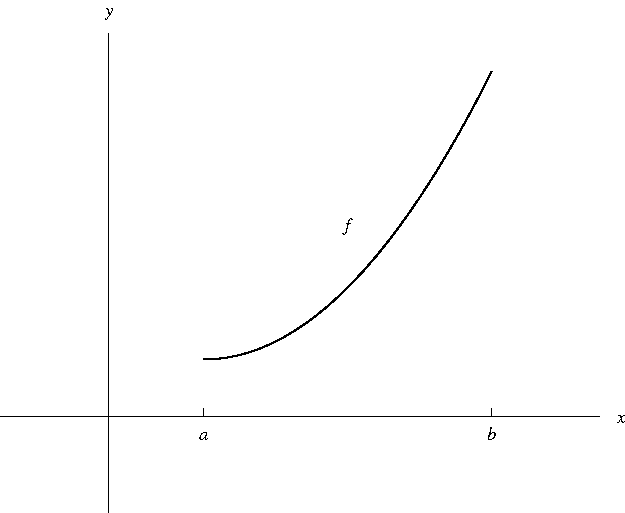
\includegraphics[height=3.5cm]{curve-sketching/pictures/04-03-concaveupa.pdf}%
}%
\only<handout:0| 3>{%
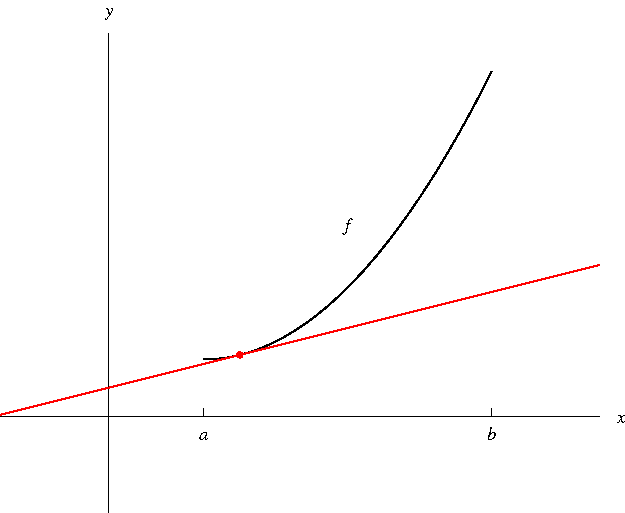
\includegraphics[height=3.5cm]{curve-sketching/pictures/04-03-concaveupb.pdf}%
}%
\only<handout:0| 4>{%
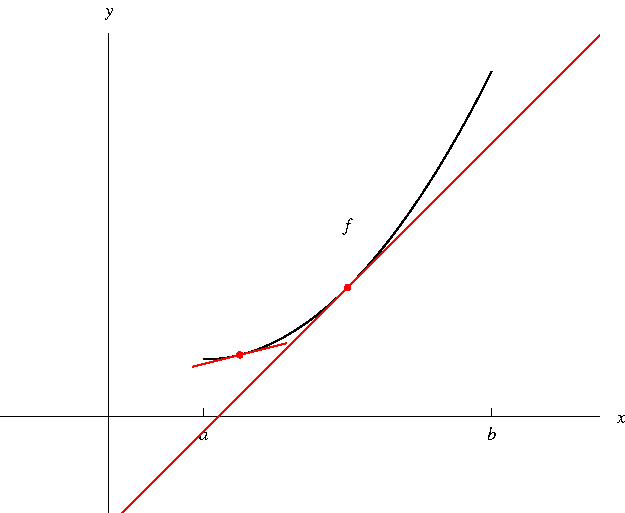
\includegraphics[height=3.5cm]{curve-sketching/pictures/04-03-concaveupc.pdf}%
}%
\only<handout:0| 5>{%
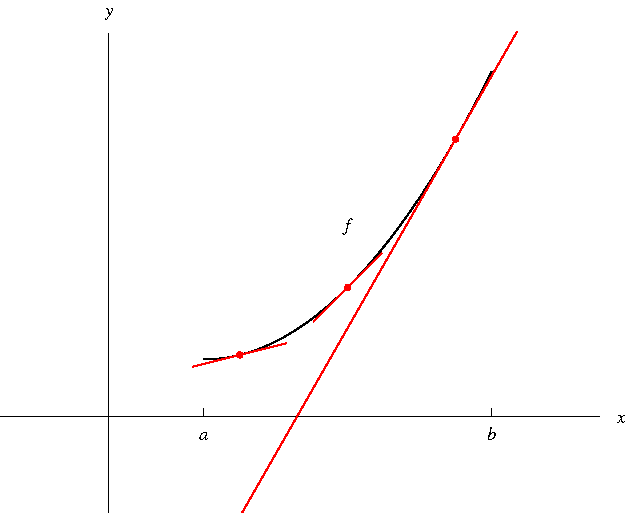
\includegraphics[height=3.5cm]{curve-sketching/pictures/04-03-concaveupd.pdf}%
}%
\only<6->{%
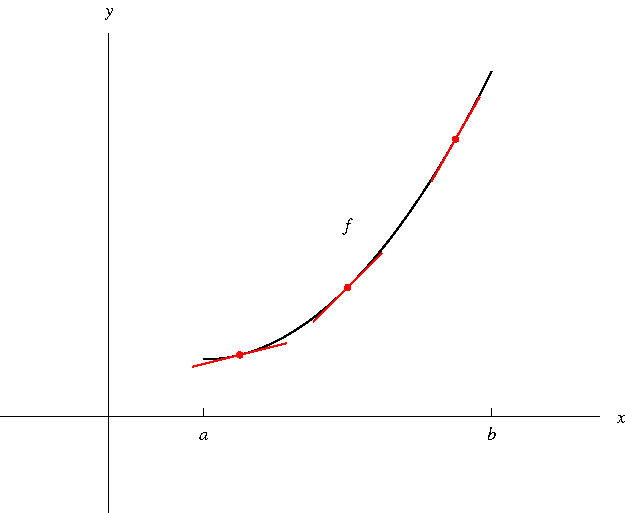
\includegraphics[height=3.5cm]{curve-sketching/pictures/04-03-concaveupe.pdf}%
}%

%\begin{center}
\ \ \ \ \ \ \ \ \ \uncover<6->{Concave up}
%\end{center}
\column{.5\textwidth}
\ \only<handout:0| -2>{%
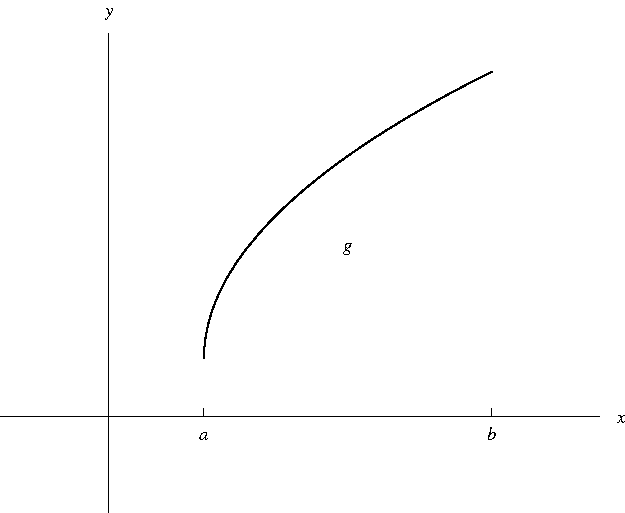
\includegraphics[height=3.5cm]{curve-sketching/pictures/04-03-concavedowna.pdf}%
}%
\only<handout:0| 3>{%
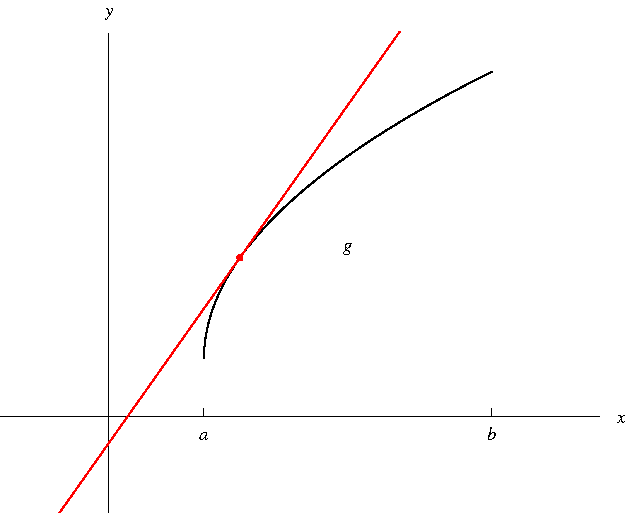
\includegraphics[height=3.5cm]{curve-sketching/pictures/04-03-concavedownb.pdf}%
}%
\only<handout:0| 4>{%
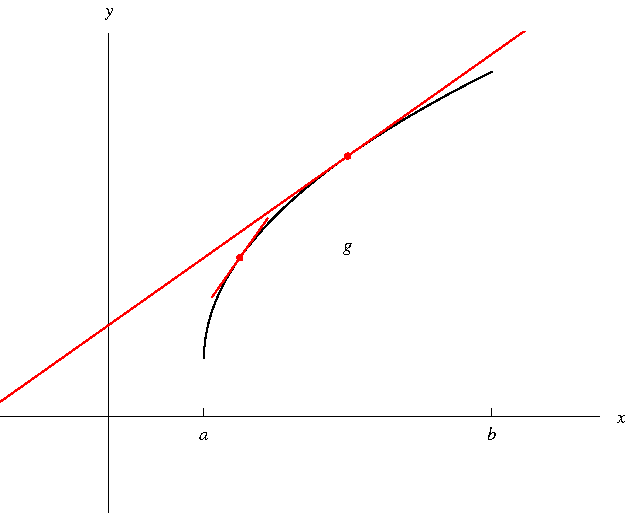
\includegraphics[height=3.5cm]{curve-sketching/pictures/04-03-concavedownc.pdf}%
}%
\only<handout:0| 5>{%
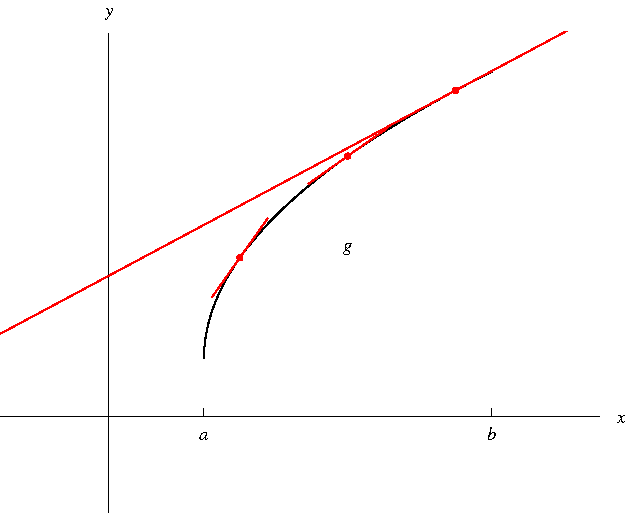
\includegraphics[height=3.5cm]{curve-sketching/pictures/04-03-concavedownd.pdf}%
}%
\only<6->{%
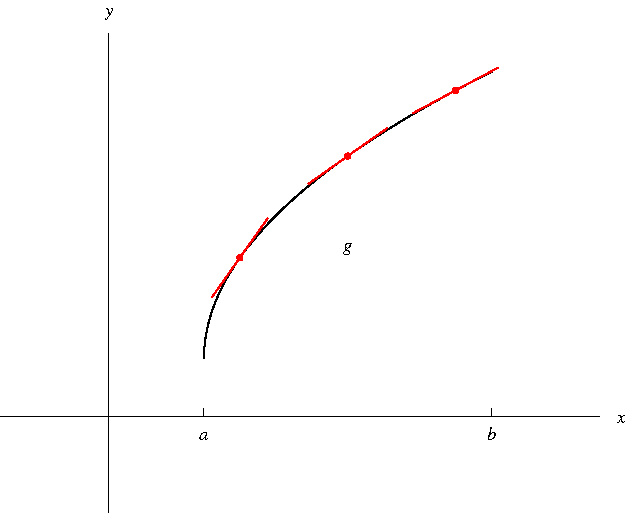
\includegraphics[height=3.5cm]{curve-sketching/pictures/04-03-concavedowne.pdf}%
}%

%\begin{center}
\ \ \ \ \ \ \ \ \ \uncover<6->{Concave down}
%\end{center}
\end{columns}
\uncover<2->{%
\begin{definition}[Concave Up/Concave Down]
If the graph of $f$ lies above all of its tangents on an interval $I$, then it is called concave up on $I$.  If it lies below all of its tangents on $I$, it is called concave down on $I$.
\end{definition}
}%
\end{frame}
% end module concavity-def

% end lecture

\end{document}
